\documentclass[11pt]{standalone}
\usepackage{amssymb}
\usepackage{amsmath}
\usepackage[no-math]{fontspec}
\usepackage{unicode-math}
\setmainfont{Libertinus Sans}
\setsansfont{Libertinus Sans}
\setmathfont{Libertinus Math}
\usepackage{pgf,xcolor}
\usepackage{tikz}
\usetikzlibrary{arrows.meta, backgrounds}
\usepackage{pgfplots}
\pgfplotsset{compat=newest}
\usepackage{pifont}

\definecolor{my_darkgray}{HTML}{484949}
\definecolor{my_lightgray}{HTML}{F3F4F4}
\definecolor{my_darkblue}{HTML}{005A94}
\definecolor{my_lightblue}{HTML}{CCDEE9}
\definecolor{my_yellow}{HTML}{FFEC7F}
\definecolor{my_red}{HTML}{E60000}
\definecolor{my_orange}{HTML}{E87846}

\begin{document}

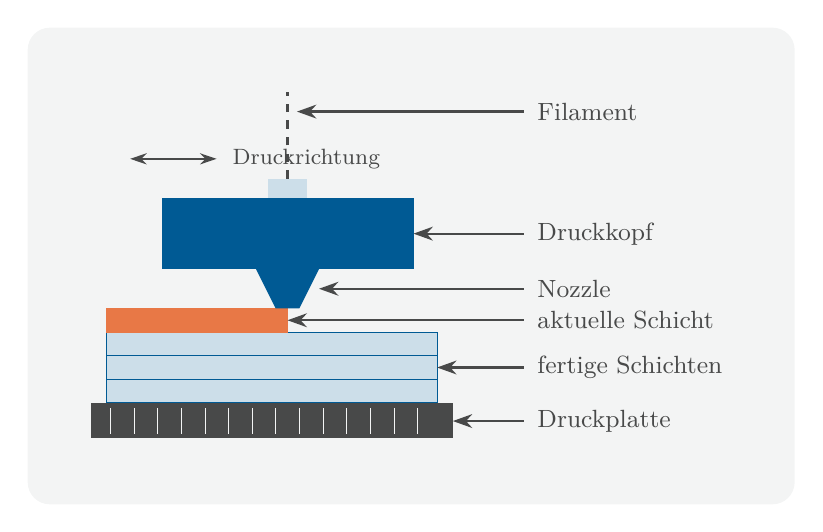
\begin{tikzpicture}[
    show background rectangle,
    background rectangle/.style={fill=my_lightgray, rounded corners=8pt},
    inner frame sep=0.8cm,
    annotation/.style={draw=my_darkgray, thick, -{Stealth[length=7pt, width=5pt]}}
]

%% ---- Druckplatte ----
\fill[fill=my_darkgray]
    (0, 0) rectangle (4.6, 0.45);
%% Subtile Oberflaechen-Textur der Druckplatte
\foreach \x in {0.25, 0.55, ..., 4.45} {
    \draw[draw=my_lightgray, very thin] (\x, 0.06) -- (\x, 0.39);
}

%% ---- Fertige Schichten (3 Stueck) ----
\fill[fill=my_lightblue, draw=my_darkblue, thin]
    (0.2, 0.45) rectangle (4.4, 0.75);
\fill[fill=my_lightblue, draw=my_darkblue, thin]
    (0.2, 0.75) rectangle (4.4, 1.05);
\fill[fill=my_lightblue, draw=my_darkblue, thin]
    (0.2, 1.05) rectangle (4.4, 1.35);

%% ---- Aktuelle Schicht (teilweise gedruckt) ----
\fill[fill=my_orange, draw=my_orange]
    (0.2, 1.35) rectangle (2.5, 1.65);

%% ---- Nozzle (Trapezform: unten schmal, oben breit) ----
%%     Unterseite: x = 2.35 bis 2.65  bei y = 1.65
%%     Oberseite:  x = 2.10 bis 2.90  bei y = 2.15
\fill[fill=my_darkblue]
    (2.10, 2.15) -- (2.90, 2.15)
    -- (2.65, 1.65) -- (2.35, 1.65) -- cycle;

%% ---- Druckkopf (Carriage-Block) ----
\fill[fill=my_darkblue]
    (0.9, 2.15) rectangle (4.1, 3.05);

%% ---- Filament-Einlass (kleiner Kanal oben am Druckkopf) ----
\fill[fill=my_lightblue]
    (2.25, 3.05) rectangle (2.75, 3.30);

%% ---- Filament (gestrichelte vertikale Linie) ----
\draw[draw=my_darkgray, dashed, line width=0.9pt]
    (2.50, 3.30) -- (2.50, 4.40);

%% ---- Bewegungsrichtung des Druckkopfs ----
\draw[draw=my_darkgray, thick,
      {Stealth[length=6pt, width=4pt]}-{Stealth[length=6pt, width=4pt]}]
    (0.50, 3.55) -- (1.60, 3.55);
\node[font=\footnotesize, text=my_darkgray, anchor=west]
    at (1.68, 3.55) {Druckrichtung};

%% ================================================================
%% Annotationen (alle rechts, Pfeile zeigen nach links zum Objekt)
%% ================================================================

%% Filament
\draw[annotation] (5.5, 4.15) -- (2.62, 4.15);
\node[font=\small, text=my_darkgray, anchor=west]
    at (5.55, 4.15) {Filament};

%% Druckkopf
\draw[annotation] (5.5, 2.60) -- (4.10, 2.60);
\node[font=\small, text=my_darkgray, anchor=west]
    at (5.55, 2.60) {Druckkopf};

%% Nozzle (Pfeil auf Mitte der Trapezform)
\draw[annotation] (5.5, 1.90) -- (2.90, 1.90);
\node[font=\small, text=my_darkgray, anchor=west]
    at (5.55, 1.90) {Nozzle};

%% Aktuelle Schicht (Pfeil auf rechten Rand der orangen Schicht)
\draw[annotation] (5.5, 1.50) -- (2.50, 1.50);
\node[font=\small, text=my_darkgray, anchor=west]
    at (5.55, 1.50) {aktuelle Schicht};

%% Fertige Schichten (Pfeil auf rechten Rand der mittleren Schicht)
\draw[annotation] (5.5, 0.90) -- (4.40, 0.90);
\node[font=\small, text=my_darkgray, anchor=west]
    at (5.55, 0.90) {fertige Schichten};

%% Druckplatte (Pfeil auf rechten Rand der Platte)
\draw[annotation] (5.5, 0.22) -- (4.60, 0.22);
\node[font=\small, text=my_darkgray, anchor=west]
    at (5.55, 0.22) {Druckplatte};

\end{tikzpicture}

\end{document}
